\section{Implementación}

Utilizando el sistema de escenas que ofrece el motor \Gls{unity}, se implementó cada espacio del videojuego como su propio nivel independiente. De esta forma se pudo implementar, probar, y pulir cada mecánica de forma aislada sin afectar al resto del juego. En la Figura~\ref{fig:escenas-general} se ve un esquema de las escenas utilizadas en general. En la Figura~\ref{fig:escenas-viva} se muestran las escenas usadas en la ruta viva y en la Figura~\ref{fig:escenas-muerta} las usadas en la ruta muerta.

\begin{figure}[h]
    \centering
    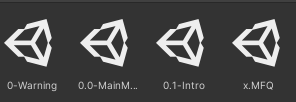
\includegraphics{imgs/unity1.png}
    \caption{Escenas Generales}
    \label{fig:escenas-general}
\end{figure}
\begin{figure}[h]
    \centering
    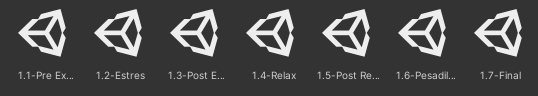
\includegraphics{imgs/unity2.png}
    \caption{Escenas Ruta Viva}
    \label{fig:escenas-viva}
\end{figure}
\begin{figure}[h]
    \centering
    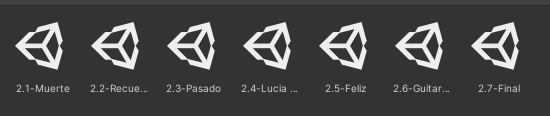
\includegraphics{imgs/unity3.png}
    \caption{Escenas Ruta Muerta}
    \label{fig:escenas-muerta}
\end{figure}

\subsection{Diagramas de clases}

Esta independencia se ve también en las clases creadas. Se generaron paquetes independientes para cada minijuego y para el sistema de diálogos, los cuales contienen las clases necesarias para que cada espacio funcione adecuadamente, como se ve en la Figura~\ref{fig:diagrama-clases}.

\begin{figure}[h]
    \centering
    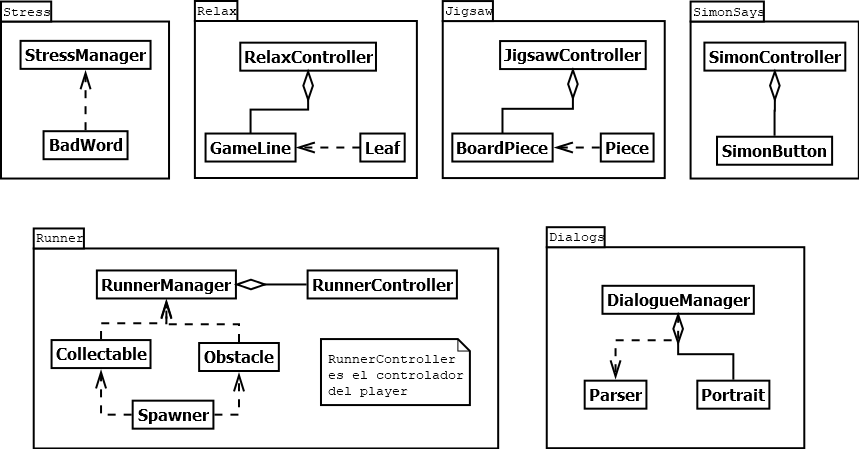
\includegraphics[width=\textwidth]{imgs/diagrama_clases.png}
    \caption{Diagrama de Clases Minijuegos}
    \label{fig:diagrama-clases}
\end{figure}

\begin{figure}[h]
    \centering
    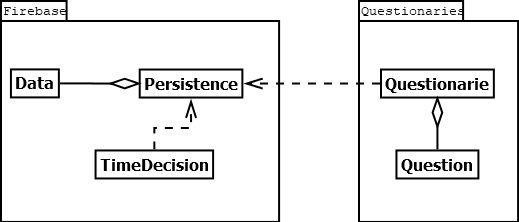
\includegraphics[scale=0.7]{imgs/diagrama_encuesta.png}
    \caption{Diagrama de Clases \Gls{firebase}}
    \label{fig:clases-firebase}
\end{figure}

\subsection{Base de Datos}
Para la recolección de los datos necesaria para la investigación se utilizo la plataforma \Gls{firebase} como \gls{backend}, utilizando principalmente Realtime Database (Una base de datos no-sql) para almacenar los datos recolectados de las encuestas y las decisiones tomadas en el juego. El diagrama de clase de estos paquetes se muestra en la Figura~\ref{fig:clases-firebase}.

En este paquete, la clase \textbf{Persistence} genera la conexión para poder guardar los datos en la base de datos de \Gls{firebase}, mientras que la clase \textbf{Data} sirve de clase modelo de los datos.

\subsection{Ejemplo de Código}
De las clases anteriormente mencionadas, es importante destacar la clase \textbf{Parser}\footnote{Para la implementación completa de la clase visitar \url{https://github.com/Jfriffoa/TFG/blob/master/Assets/Scripts/Dialogs/Parser.cs}}, la cuál me permite mantener los diálogos en un documento txt separados del código, volviéndolo más modular y facilitando modificaciones en la narrativa.

\begin{lstlisting}[language={[Sharp]C}, caption={Fragmento de Parser.cs}, label={lst:parser}]
public static List<Dialog> LoadFileFromString(string txt) {
    List<Dialog> dialogs = new List<Dialog>();

    if (string.IsNullOrEmpty(txt)) {
        Debug.LogWarning("The string doesn't have data. Aborting...");
        return dialogs;
    }

    using (var reader = new StringReader(txt)) {
        int lineIdx = 0;
        string line;
        while ((line = reader.ReadLine()) != null) {
            lineIdx++;
            if (!string.IsNullOrEmpty(line) && !line.StartsWith("//"))
                dialogs.Add(ParseLine(line, lineIdx));
        }
    }

    return dialogs;
}

static Dialog ParseLine(string line, int lineIdx) {
    int idx = line.IndexOf(":");

    var (attr, p1, p2) = ParseAttributes(line.Substring(0, idx));
    var txt = line.Substring(idx + 1);

    return new Dialog(txt, attr, p1, p2, lineIdx);
}
\end{lstlisting}

\begin{figure}[h]
    \centering
    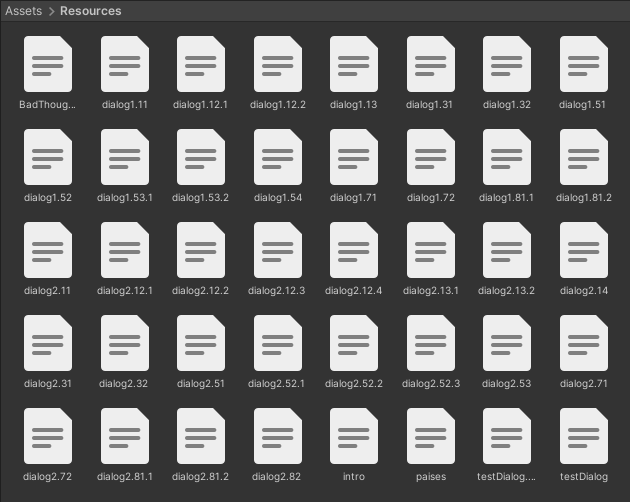
\includegraphics[scale=0.7]{imgs/unity-resources.png}
    \caption{Guión en archivos .txt}
    \label{fig:txts}
\end{figure}

\subsection{Pruebas}

Durante el tiempo de desarrollo se hicieron constantes pruebas manuales en el \gls{engine} y en el dispositivo móvil mencionado en el Cuadro~\ref{tab:movil} en la Sección~\ref{sec:recurso-tecnologico}, para ir asegurando el correcto funcionamiento de las mecánicas implementadas y del flujo general del videojuego.

Una vez el juego fue completado, se dio paso a las sesiones de prueba con usuarios reales. El \GLS{apk} del juego fue subido a \Gls{drive} para su divulgación y el sistema de testeo fue el siguiente:

\begin{center}
    \textbf{Advertencia -\textgreater  Pre-Encuesta -\textgreater  Juego -\textgreater  Post-Encuesta}
\end{center}

Exceptuando por la sección de Advertencia (que es una pantalla informativa para el usuario, donde se le indica que sus datos de juego serán recolectados de forma anónima para la realización de esta investigación) al termino de cada una de las secciones se suben los datos recolectados a la base de datos.

Para esta sesión de prueba, se divulgó el juego mediante boca a boca, compartiéndolo directamente con amigos y conocidos además de publicaciones en redes sociales, otorgando el tiempo de una semana calendario para poder llegar a la mayor cantidad de gente posible y conseguir una buena cantidad de datos.

\subsection{Confidencialidad}
La información recolectada por parte del usuario se realiza de manera totalmente anónima. Cada usuario tiene asignado un id único y se recolectan solamente los datos de juego y datos demográficos preguntados directamente a los usuarios. La Figura~\ref{fig:advertencia} muestra la pantalla de advertencia que aparece al inicio del juego.

\begin{figure}[h]
    \centering
    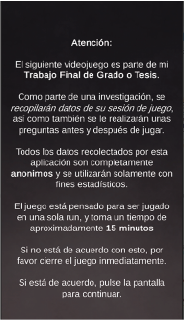
\includegraphics[scale=1.1]{imgs/advertencia.png}
    \caption{Pantalla de Información}
    \label{fig:advertencia}
\end{figure}

%\textbf{TEMA CONFIDENCIALIDAD DE LA INFORMACIÓN, es necesario tener consentimiento del usuario debe salir algun tipo de nota informativa!!!}